\documentclass[12pt,a4paper]{article}

\usepackage[utf8]{inputenc}
\usepackage[T1]{fontenc}
\usepackage[provide=*,spanish]{babel}
\usepackage{mathpazo}
\usepackage{microtype}
\usepackage{amsmath,amssymb,amsthm}
\usepackage{geometry}
\usepackage{enumitem}
\usepackage{tikz}
\usepackage{pgfplots}
\usepackage[hidelinks]{hyperref}

\usetikzlibrary{arrows.meta,calc}
\pgfplotsset{compat=1.18}
\geometry{margin=2.5cm}

\newcommand{\R}{\mathbb{R}}

\title{Ecuaciones Diferenciales Ordinarias\\Material suplementario: flujos unidimensionales y estabilidad}
\author{Benjamín Marcolongo}
\date{}

\begin{document}

	\maketitle

	\section{Propósito}

	Una ecuación autónoma escalar
	\[
	\dot{x}=f(x)
	\]
puede parecer demasiado sencilla: solo hay una variable de estado y el tiempo no aparece explícitamente. Sin embargo, este caso contiene varias ideas centrales de la teoría cualitativa de ecuaciones diferenciales: campo vectorial, flujo, puntos fijos, estabilidad y linealización.

	El objetivo es desarrollar esas ideas sin depender de la resolución explícita de cada ecuación. Estudiaremos:
	\begin{enumerate}[label=\arabic*.]
		\item cómo leer una ecuación autónoma como un campo de velocidades sobre la recta;
		\item cómo construir y utilizar una recta de fase;
		\item cómo clasificar puntos fijos mediante la linealización;
		\item qué puede decirse cuando la linealización no decide la estabilidad;
		\item cómo estas herramientas permiten comprender los modelos exponencial y logístico.
	\end{enumerate}

	En todo el material, el punto indica derivación respecto del tiempo:
	\[
	\dot{x}=\frac{dx}{dt}.
	\]

	\clearpage
	\section{Ecuaciones autónomas como campos vectoriales}

	Consideremos
	\[
	\dot{x}=f(x),
	\]
donde \(f\colon D\subseteq\R\to\R\). El valor \(f(x)\) asigna una velocidad a cada estado:
	\[
	f(x)>0 \Longrightarrow x(t)\text{ aumenta},
	\qquad
	f(x)<0 \Longrightarrow x(t)\text{ disminuye}.
	\]
Por lo tanto, \(f\) puede interpretarse como un campo vectorial unidimensional. En cada punto de la recta de estados dibujamos una flecha hacia la derecha si \(f(x)>0\) y hacia la izquierda si \(f(x)<0\).

	Esta lectura separa dos objetos que conviene no confundir:
	\begin{itemize}[leftmargin=*]
		\item la \textbf{gráfica de \(f\)}, que representa la velocidad en función del estado;
		\item las \textbf{curvas solución \(x(t)\)}, que representan la evolución del estado en el tiempo.
	\end{itemize}

	\subsection{Puntos fijos}

	Un valor \(x^\ast\in D\) es un \textbf{punto fijo}, \textbf{punto crítico} o \textbf{equilibrio} si
	\[
	f(x^\ast)=0.
	\]
En ese caso, la función constante
	\[
	x(t)=x^\ast
	\]
es una solución. Los puntos fijos dividen la recta de estados en intervalos. Si \(f\) es continua, su signo no puede cambiar dentro de uno de esos intervalos sin que aparezca otro cero; basta estudiar el signo de \(f\) en un punto de cada intervalo.

	\subsection{La recta de fase}

	La \textbf{recta de fase} reúne los puntos fijos y el sentido del movimiento. Si el signo de \(f\) es positivo a la izquierda de \(x^\ast\) y negativo a la derecha, las flechas apuntan hacia \(x^\ast\):
	\begin{center}
	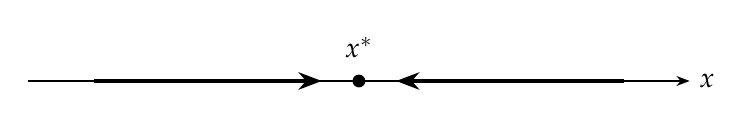
\begin{tikzpicture}[>=Stealth,scale=1.05]
		\draw[->] (-4,0)--(4,0) node[right] {$x$};
		\fill (0,0) circle (2.2pt) node[above=5pt] {$x^\ast$};
		\draw[->,very thick] (-3.2,0)--(-0.45,0);
		\draw[->,very thick] (3.2,0)--(0.45,0);
	\end{tikzpicture}
	\end{center}
El equilibrio atrae las trayectorias cercanas. Si las flechas apuntan hacia afuera, las perturbaciones se alejan y el equilibrio es inestable. Si una flecha apunta hacia el equilibrio y la otra se aleja, el punto es \textbf{semiestable}.

	\begin{quote}
		\textbf{Idea central.} En una dimensión, la dinámica cualitativa está determinada esencialmente por el orden de los puntos fijos y el signo de \(f\) entre ellos.
	\end{quote}

	\clearpage
	\section{Ejemplo: el flujo generado por el seno}

	Los puntos fijos de
	\[
	\dot{x}=\sin x
	\]
satisfacen
	\[
	x_k^\ast=k\pi,
	\qquad k\in\mathbb{Z}.
	\]
El signo del seno alterna entre ceros consecutivos. La recta de fase es periódica:
	\begin{center}
	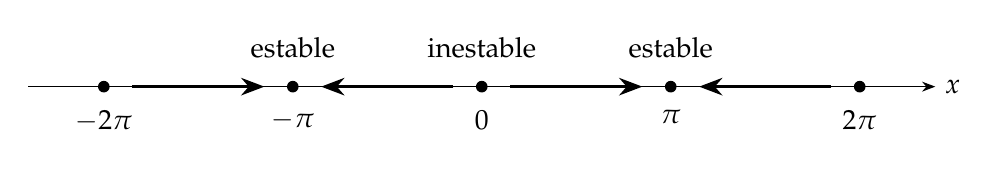
\begin{tikzpicture}[>=Stealth,x=1.2cm,y=1cm]
		\draw[->] (-4.8,0)--(4.8,0) node[right] {$x$};
		\foreach \x/\lab in {-4/{-2\pi},-2/{-\pi},0/{0},2/{\pi},4/{2\pi}}{
			\fill (\x,0) circle (2.1pt) node[below=5pt] {$\lab$};
		}
		\draw[->,very thick] (-3.7,0)--(-2.3,0);
		\draw[->,very thick] (-0.3,0)--(-1.7,0);
		\draw[->,very thick] (0.3,0)--(1.7,0);
		\draw[->,very thick] (3.7,0)--(2.3,0);
		\node[above=7pt] at (-2,0) {estable};
		\node[above=7pt] at (0,0) {inestable};
		\node[above=7pt] at (2,0) {estable};
	\end{tikzpicture}
	\end{center}
Los equilibrios \(x=(2k+1)\pi\) son atractores, mientras que \(x=2k\pi\) son repulsores.

	\subsection{Resolución explícita}

	En un intervalo que no contenga un cero de \(\sin x\), separamos variables:
	\[
	\frac{dx}{\sin x}=dt.
	\]
Como
	\[
	\int\csc x\,dx
	=
	\ln\left|\tan\frac{x}{2}\right|+C,
	\]
se obtiene
	\[
	\ln\left|\tan\frac{x}{2}\right|=t+C.
	\]
Si \(x(0)=x_0\notin\pi\mathbb{Z}\), entonces
	\[
	\tan\frac{x(t)}{2}
	=
	\tan\frac{x_0}{2}\,e^t.
	\]
Por lo tanto,
	\[
	x(t)
	=
	2\arctan\left(\tan\frac{x_0}{2}\,e^t\right)+2k\pi,
	\]
donde debe elegirse \(k\) para que la expresión permanezca en el mismo intervalo delimitado por puntos fijos que contiene a \(x_0\). La elección de rama es parte de la solución: las trayectorias no atraviesan un equilibrio cuando hay unicidad.

	Por ejemplo, si \(0<x_0<\pi\),
	\[
	\lim_{t\to-\infty}x(t)=0,
	\qquad
	\lim_{t\to\infty}x(t)=\pi.
	\]
La trayectoria abandona el equilibrio inestable \(0\) hacia el pasado y se aproxima al equilibrio estable \(\pi\) hacia el futuro.

	\clearpage
	\section{Definiciones de estabilidad}

	Sea \(x^\ast\) un punto fijo de \(\dot{x}=f(x)\).

	\subsection{Estabilidad de Lyapunov}

	El punto fijo \(x^\ast\) es \textbf{estable} si para todo \(\varepsilon>0\) existe \(\delta>0\) tal que
	\[
	|x(0)-x^\ast|<\delta
	\]
implica
	\[
	|x(t)-x^\ast|<\varepsilon
	\qquad\text{para todo }t\geq 0.
	\]
Una perturbación pequeña produce una respuesta que permanece pequeña. Esto no exige que la solución vuelva al equilibrio.

	\subsection{Estabilidad asintótica}

	El punto fijo \(x^\ast\) es \textbf{asintóticamente estable} si es estable y, además, las soluciones que comienzan suficientemente cerca satisfacen
	\[
	\lim_{t\to\infty}x(t)=x^\ast.
	\]
En este caso, el equilibrio retiene y atrae las trayectorias cercanas. Un punto fijo es \textbf{inestable} cuando no es estable.

	\subsection{Estabilidad local y global}

	La clasificación anterior es local. Un equilibrio es \textbf{globalmente asintóticamente estable} en un dominio \(D\) si todas las soluciones con condición inicial en \(D\) existen para \(t\geq0\) y convergen hacia él.

	La condición de existencia global no es decorativa. Puede haber soluciones que escapen a infinito en tiempo finito y, por lo tanto, no estén definidas para todo \(t\geq0\).

	\clearpage
	\section{Análisis de estabilidad lineal}

	Sea \(x^\ast\) un punto fijo:
	\[
	f(x^\ast)=0.
	\]
Introducimos la perturbación
	\[
	\eta(t)=x(t)-x^\ast.
	\]
Como \(x^\ast\) es constante,
	\[
	\dot{\eta}=\dot{x}=f(x^\ast+\eta).
	\]
Si \(f\) es suficientemente regular, Taylor alrededor de \(x^\ast\) da
	\[
	f(x^\ast+\eta)
	=
	f(x^\ast)+f'(x^\ast)\eta+O(\eta^2).
	\]
Como \(f(x^\ast)=0\),
	\[
	\dot{\eta}
	=
	f'(x^\ast)\eta+O(\eta^2).
	\]
La \textbf{ecuación linealizada} es
	\[
	\dot{\eta}=f'(x^\ast)\eta,
	\]
cuya solución es
	\[
	\eta(t)=\eta_0e^{f'(x^\ast)t}.
	\]
Por lo tanto,
	\[
	\boxed{
	\begin{aligned}
	f'(x^\ast)<0&\quad\Longrightarrow\quad x^\ast\text{ es asintóticamente estable},\\
	f'(x^\ast)>0&\quad\Longrightarrow\quad x^\ast\text{ es inestable}.
	\end{aligned}}
	\]
Geométricamente, una pendiente negativa implica que \(f\) cruza el eje con velocidades dirigidas hacia el cero; una pendiente positiva produce velocidades dirigidas hacia afuera.

	\subsection{Aplicación al seno}

	Para \(f(x)=\sin x\),
	\[
	f'(x)=\cos x.
	\]
En \(x_k^\ast=k\pi\),
	\[
	f'(x_k^\ast)=\cos(k\pi)=(-1)^k.
	\]
Si \(k\) es par, la derivada vale \(1\) y el equilibrio es inestable. Si \(k\) es impar, vale \(-1\) y el equilibrio es asintóticamente estable.

	\clearpage
	\section{Cuando la linealización no decide}

	Si
	\[
	f'(x^\ast)=0,
	\]
la ecuación linealizada es \(\dot{\eta}=0\). Esto no prueba estabilidad ni inestabilidad: el término lineal no contiene información suficiente. Deben examinarse los términos no lineales o el signo de \(f\) a ambos lados del equilibrio.

	Supongamos que el primer término no nulo es
	\[
	\dot{\eta}=a\eta^m+O(\eta^{m+1}),
	\qquad a\neq0,\quad m\geq2.
	\]
Entonces:
	\begin{itemize}[leftmargin=*]
		\item si \(m\) es impar y \(a<0\), el equilibrio es asintóticamente estable;
		\item si \(m\) es impar y \(a>0\), el equilibrio es inestable;
		\item si \(m\) es par, el equilibrio es semiestable.
	\end{itemize}

	Por ejemplo, para
	\[
	\dot{x}=-x^3,
	\]
se cumple \(f'(0)=0\), pero las flechas apuntan hacia \(0\) desde ambos lados: el origen es asintóticamente estable. En cambio, para
	\[
	\dot{x}=x^2,
	\]
también se cumple \(f'(0)=0\), pero \(f(x)>0\) a ambos lados: el origen atrae desde la izquierda y repele desde la derecha.

	\begin{quote}
		\textbf{Advertencia.} El criterio basado en \(f'(x^\ast)\) es concluyente cuando la derivada es distinta de cero. Cuando vale cero, no debe concluirse que el equilibrio sea estable.
	\end{quote}

	\clearpage
	\section{Ejemplo completo: dos puntos fijos}

	Los puntos fijos son
	\[
	x^\ast=-1,
	\qquad
	x^\ast=1.
	\]
Como
	\[
	f'(x)=2x,
	\]
se tiene
	\[
	f'(-1)=-2<0,
	\qquad
	f'(1)=2>0.
	\]
Así, \(x=-1\) es asintóticamente estable y \(x=1\) es inestable. La misma conclusión se obtiene factorizando \(f(x)=(x-1)(x+1)\):
	\begin{center}
	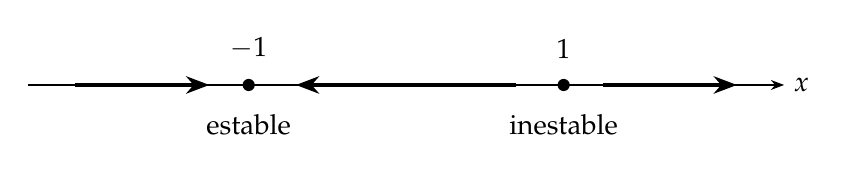
\begin{tikzpicture}[>=Stealth,x=2cm]
		\draw[->] (-2.4,0)--(2.4,0) node[right] {$x$};
		\fill (-1,0) circle (2.2pt) node[above=6pt] {$-1$};
		\fill (1,0) circle (2.2pt) node[above=6pt] {$1$};
		\draw[->,very thick] (-2.1,0)--(-1.25,0);
		\draw[->,very thick] (0.7,0)--(-0.7,0);
		\draw[->,very thick] (1.25,0)--(2.1,0);
		\node[below=7pt] at (-1,0) {estable};
		\node[below=7pt] at (1,0) {inestable};
	\end{tikzpicture}
	\end{center}

	\subsection{Solución explícita y existencia global}

	Para soluciones no constantes,
	\[
	\frac{dx}{x^2-1}=dt.
	\]
Integrando,
	\[
	\frac12\ln\left|\frac{x-1}{x+1}\right|=t+C.
	\]
Si \(x(0)=x_0\neq\pm1\),
	\[
	x(t)=\frac{1+Ce^{2t}}{1-Ce^{2t}},
	\qquad
	C=\frac{x_0-1}{x_0+1}.
	\]
Para \(-1<x_0<1\), la solución converge a \(-1\). Para \(x_0<-1\), también converge a \(-1\) hacia el futuro. Si \(x_0>1\), el denominador se anula en
	\[
	t_\ast=\frac12\ln\left(\frac{x_0+1}{x_0-1}\right),
	\]
y la solución diverge en tiempo finito. El retrato de fase también puede revelar la ausencia de existencia global.

	\clearpage
	\section{Del crecimiento exponencial al modelo logístico}

	Sea \(N(t)\) el tamaño de una población. El supuesto más sencillo es que, durante un intervalo pequeño \(\Delta t\), el cambio sea proporcional a la población presente:
	\[
	N(t+\Delta t)-N(t)
	\approx
	rN(t)\Delta t.
	\]
Dividiendo por \(\Delta t\) y tomando el límite \(\Delta t\to0\),
	\[
	\dot{N}=rN.
	\]
Su solución es
	\[
	N(t)=N_0e^{rt}.
	\]
Si \(r>0\), la población crece sin cota; si \(r=0\), permanece constante; si \(r<0\), decae exponencialmente.

	El crecimiento exponencial no incorpora la competencia por recursos. El modelo logístico supone que la tasa de crecimiento per cápita disminuye linealmente con \(N\):
	\[
	\frac{\dot{N}}{N}
	=
	r\left(1-\frac{N}{K}\right),
	\]
donde \(r>0\) es la tasa intrínseca y \(K>0\) la \textbf{capacidad de carga}. Así se obtiene
	\[
	\boxed{\dot{N}=rN\left(1-\frac{N}{K}\right).}
	\]

	El factor \(N\) expresa que la producción total de nuevos individuos es proporcional al número presente. El factor \(1-N/K\) representa la limitación ambiental:
	\[
	\begin{array}{ccl}
	0<N<K &\Longrightarrow& \dot N>0,\\[1mm]
	N=K   &\Longrightarrow& \dot N=0,\\[1mm]
	N>K   &\Longrightarrow& \dot N<0.
	\end{array}
	\]
El modelo no afirma que el crecimiento se detenga bruscamente al alcanzar \(K\); la tasa neta disminuye progresivamente y se anula allí.

	\clearpage
	\section{Análisis cualitativo del modelo logístico}

	Definamos
	\[
	f(N)=rN\left(1-\frac{N}{K}\right).
	\]
Los puntos fijos son \(N^\ast=0\) y \(N^\ast=K\). Como
	\[
	f'(N)=r\left(1-\frac{2N}{K}\right),
	\]
resulta
	\[
	f'(0)=r>0,
	\qquad
	f'(K)=-r<0.
	\]
Por lo tanto, \(N=0\) es inestable y \(N=K\) es asintóticamente estable para \(r>0\).

	\begin{center}
	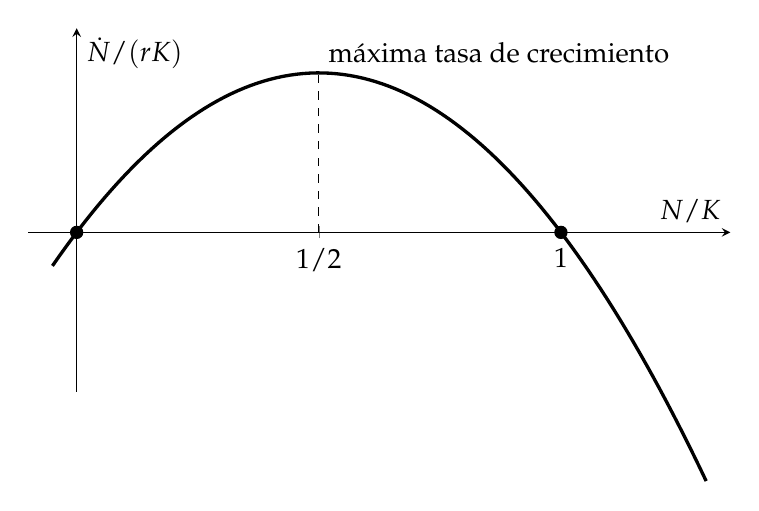
\begin{tikzpicture}
	\begin{axis}[
		width=10.5cm,height=6.2cm,
		axis lines=middle,
		xmin=-0.1,xmax=1.35,
		ymin=-0.25,ymax=0.32,
		xlabel={$N/K$},ylabel={$\dot N/(rK)$},
		xtick={0,0.5,1},xticklabels={$0$,$1/2$,$1$},
		ytick=\empty,clip=false
	]
		\addplot[very thick,domain=-0.05:1.3,samples=100] {x*(1-x)};
		\addplot[only marks,mark=*,mark size=2.2pt] coordinates {(0,0) (1,0)};
		\draw[dashed] (axis cs:0.5,0)--(axis cs:0.5,0.25);
		\node[above right] at (axis cs:0.5,0.25) {máxima tasa de crecimiento};
	\end{axis}
	\end{tikzpicture}
	\end{center}

	La velocidad de crecimiento es máxima en \(N=K/2\). Derivando respecto del tiempo,
	\[
	\ddot N=f'(N)\dot N.
	\]
Para una solución con \(0<N<K\), se cumple \(\dot N>0\), y el cambio de concavidad ocurre cuando
	\[
	f'(N)=0
	\quad\Longleftrightarrow\quad
	N=\frac K2.
	\]
Antes de alcanzar \(K/2\), la curva es cóncava hacia arriba; después es cóncava hacia abajo.

	\subsection{Solución explícita}

	Separando variables e imponiendo \(N(0)=N_0>0\),
	\[
	N(t)
	=
	\frac{K}{1+A e^{-rt}},
	\qquad
	A=\frac{K-N_0}{N_0}.
	\]
Si \(0<N_0<K\), la población crece hacia \(K\). Si \(N_0>K\), decrece hacia \(K\). En ambos casos,
	\[
	\lim_{t\to\infty}N(t)=K.
	\]

	\subsection{Retrato de las soluciones}

	\begin{center}
	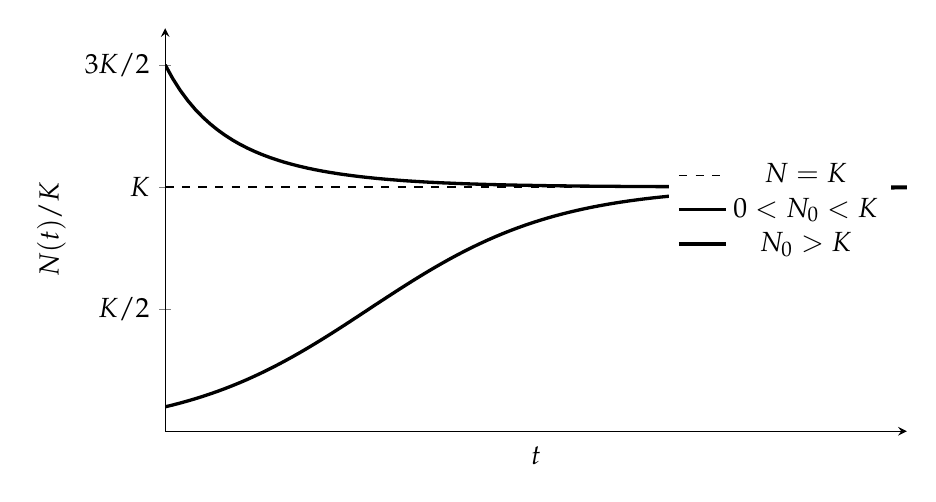
\begin{tikzpicture}
	\begin{axis}[
		width=11cm,height=6.7cm,
		axis lines=left,
		xmin=0,xmax=8,ymin=0,ymax=1.65,
		xlabel={$t$},ylabel={$N(t)/K$},
		ytick={0.5,1,1.5},yticklabels={$K/2$,$K$,$3K/2$},
		xtick=\empty,
		legend style={draw=none,at={(0.98,0.55)},anchor=east}
	]
		\addplot[dashed] coordinates {(0,1) (8,1)};
		\addplot[very thick,domain=0:8,samples=100] {1/(1+9*exp(-x))};
		\addplot[very thick,domain=0:8,samples=100] {1/(1-0.333333*exp(-x))};
		\legend{$N=K$,$0<N_0<K$,$N_0>K$}
	\end{axis}
	\end{tikzpicture}
	\end{center}

	El semieje \(N\geq0\) es invariante: una población inicialmente no negativa no se vuelve negativa. Esto se sigue de la unicidad, porque una solución con \(N_0>0\) no puede atravesar la solución de equilibrio \(N=0\). Del mismo modo, las soluciones que comienzan por debajo de \(K\) no lo sobrepasan, y las que comienzan por encima no lo cruzan.

	Para \(N_0>0\), todas las soluciones existen para todo \(t\geq0\) y convergen a \(K\). Por eso \(K\) es globalmente asintóticamente estable en el dominio biológicamente relevante \(N>0\), aunque no lo sea en toda la recta real.

	\subsection{Adimensionalización}

	Las variables
	\[
	u=\frac{N}{K},
	\qquad
	\tau=rt
	\]
transforman el modelo en
	\[
	\frac{du}{d\tau}=u(1-u).
	\]
Así, \(K\) fija la escala poblacional y \(1/r\) fija la escala temporal. Una vez expresadas las variables en estas unidades, todos los modelos logísticos con \(r,K>0\) poseen el mismo retrato de fase.

	\clearpage
	\section{Modelo continuo, modelo discreto y limitaciones}

	El modelo logístico continuo trata \(N(t)\) como una variable real y distribuye nacimientos y muertes continuamente en el tiempo. Es razonable para poblaciones grandes con generaciones superpuestas, pero no para toda población biológica.

	Una discretización de Euler con paso \(\Delta t\) produce
	\[
	N_{n+1}
	=
	N_n+r\Delta t\,N_n\left(1-\frac{N_n}{K}\right).
	\]
Cuando \(\Delta t\) es pequeño, esta recurrencia aproxima el flujo continuo. Para pasos grandes puede presentar oscilaciones e incluso valores negativos que no corresponden al comportamiento de la EDO.

	El \textbf{mapa logístico},
	\[
	u_{n+1}=\lambda u_n(1-u_n),
	\]
es un modelo discreto relacionado, pero no es simplemente la misma dinámica observada en tiempos enteros. Dependiendo de \(\lambda\), puede exhibir ciclos y caos. En cambio, una EDO autónoma escalar no puede tener órbitas periódicas no constantes: dentro de cada intervalo sin puntos fijos, el signo de \(\dot x\) es constante y las soluciones son monótonas.

	El modelo logístico también supone:
	\begin{itemize}[leftmargin=*]
		\item una capacidad de carga \(K\) constante;
		\item una población homogénea, sin estructura de edades ni espacial;
		\item respuesta instantánea a la densidad, sin retardos;
		\item ausencia de fluctuaciones ambientales y demográficas;
		\item una relación lineal entre tasa per cápita y densidad.
	\end{itemize}
Estas hipótesis determinan su dominio de validez y señalan qué mecanismos incorporar cuando las observaciones no concuerdan con el modelo.

	\clearpage
	\section{Síntesis y procedimiento de análisis}

	Para estudiar
	\[
	\dot{x}=f(x),
	\]
conviene:
	\begin{enumerate}[label=\arabic*.]
		\item determinar el dominio de \(f\);
		\item encontrar los puntos fijos resolviendo \(f(x)=0\);
		\item estudiar el signo de \(f\) entre puntos fijos;
		\item construir la recta de fase;
		\item clasificar localmente cada equilibrio;
		\item usar \(f'(x^\ast)\) cuando sea distinto de cero;
		\item si \(f'(x^\ast)=0\), estudiar el signo de \(f\) o el primer término no lineal;
		\item analizar existencia global, singularidades y límites cuando \(t\to\infty\);
		\item resolver explícitamente solo si la fórmula aporta información adicional.
	\end{enumerate}

	\begin{quote}
		\textbf{Idea final.} Resolver una EDO no significa únicamente hallar una fórmula. En muchos problemas, la recta de fase y la estabilidad describen el comportamiento global con mayor claridad que la solución explícita.
	\end{quote}

	\section*{Ejercicios propuestos}

	\begin{enumerate}[label=\arabic*.]
		\item Construya la recta de fase de \(\dot{x}=x(1-x)(x-2)\) y clasifique sus puntos fijos.
		\item Estudie la estabilidad del origen para \(\dot{x}=x^3\), \(\dot{x}=-x^5\) y \(\dot{x}=x^4\).
		\item Para el modelo logístico, determine el tiempo necesario para pasar de \(N_0=K/10\) a \(N=K/2\).
		\item Explique por qué dos soluciones distintas con unicidad no pueden cruzarse.
		\item Muestre que una solución no constante de \(\dot{x}=f(x)\) no puede ser periódica.
	\end{enumerate}

\end{document}
